% \iffalse meta-comment
% 
% Copyright (c) 2013 by Tobias Weh
%                       www.tobias-weh.de
% 
% This file may be distributed and/or modified under the 
% conditions of the LaTeX Project Public License, either 
% version 1.2 of this license or (at your option) any later 
% version. The latest version of this license is in: 
%
%	http://www.latex-project.org/lppl.txt 
% 
% and version 1.2 or later is part of all distributions of 
% LaTeX version 1999/12/01 or later.
%
% \fi
%
% \iffalse
%<package>\NeedsTeXFormat{LaTeX2e}[2009/01/01]
%<package>\ProvidesPackage{menukeys}
%<package>  [2016/04/18 v1.4 -- A package to format menus, paths and shortcuts]
%
%<*driver>
\documentclass{ltxdoc}

\usepackage[T1]{fontenc}
\usepackage[latin1]{inputenc}
\usepackage{lmodern}
\usepackage[english]{babel}
\usepackage{menukeys}
\usepackage{xspace}
\usepackage{lmodern}
\usepackage[hang]{footmisc}
\usepackage{dblfnote}
\setlength{\footnotemargin}{1em}
\usepackage{listings}
\usepackage{xcolor}
\definecolor{darkred}{HTML}{770011}
\definecolor{darkblue}{HTML}{003b8b}
\PassOptionsToPackage{%
   linkcolor=darkblue,
   urlcolor=darkred,
   bookmarksopen=true,
   bookmarksdepth=10,
}{hyperref}
\PassOptionsToPackage{hyphens}{url}
\usepackage{hypdoc}


\renewcommand{\usage}[1]{\textbf{\hyperpage{#1}}}
\renewcommand{\main}[1]{\textit{#1}}

\newcommand{\menukeys}{\texttt{menukeys}\xspace}
\newcommand{\TikZ}{Ti\textit{k}Z\xspace}

\newcommand*{\pkg}[1]{\texttt{#1}}
\newcommand*{\env}[1]{\texttt{#1}}
\newcommand*{\fnt}[1]{\texttt{#1}}
\newcommand*{\opt}[1]{\texttt{#1}}
\newcommand{\DO}[1]{%
   \marginpar{\raggedleft\texttt{#1} \footnotesize(opt.)}%
   \index{#1=\texttt{#1}  (option)|usage}%
   \index{Options:>\texttt{#1}|usage}%
   \ignorespaces
}
\newcommand{\DM}[1]{\DescribeMacro{#1}\ignorespaces}
\newcommand{\DE}[1]{\DescribeEnv{#1}\ignorespaces}
\newcommand{\AST}{\meta{\texttt{*}}}

\newcommand{\minisec}[1]{\par\medskip\noindent{\sffamily\bfseries#1}\quad}
\newcommand{\example}{\minisec{Example}\xspace}

\providemenumacro{\test}{roundedmenus}
\NewDocumentCommand{\teststyle}{ o m m m }{{%
   \renewmenumacro{\test}{#2}%
   \par\vspace{1.5\baselineskip plus 0.5\baselineskip minus 0.25\baselineskip}
   \noindent
   \fbox{\begin{minipage}{0.97\textwidth}
   Name: \texttt{#2}
      \index{#2=\texttt{#2}  (style)|usage}%
      \index{Styles:>\texttt{#2}|usage}
   \par\vspace{0.5\baselineskip}%
   \test{#3}
   \par\vspace{0.5\baselineskip}%
   \test{#4}%
   \par\vspace{0.5\baselineskip}%
   This is some more or less blind text, to demonstrate how
   the sequence looks in text. This \test{#3} is the result
   of a style which name is \texttt{#2}. And again some
   blind text without any sense.%
   \IfValueT{#1}{{%
      \par\vspace{0.5\baselineskip}%
      \itshape\footnotesize#1\par
   }}%
   \end{minipage}}%
}}
\makeatletter
\newcommand{\colortest}[1]{{%
   \par\vspace{\baselineskip}%
   \setlength{\fboxsep}{0pt}%
   \noindent Name: \texttt{#1}\index{#1=\texttt{#1}  (theme)|usage}%
   \index{Color themes:>\texttt{#1}|usage}
   \\[0.5\baselineskip]
   Background: \fbox{\textcolor{tw@color@theme@#1@bg}{\rule[-0.4ex]{2.2ex}{2.2ex}}}
   \quad Border: \fbox{\textcolor{tw@color@theme@#1@br}{\rule[-0.4ex]{2.2ex}{2.2ex}}}
   \quad Text: \fbox{\textcolor{tw@color@theme@#1@txt}{\rule[-0.4ex]{2.2ex}{2.2ex}}}
   \quad (A: \fbox{\textcolor{tw@color@theme@#1@a}{\rule[-0.4ex]{2.2ex}{2.2ex}}}
   \quad B: \fbox{\textcolor{tw@color@theme@#1@b}{\rule[-0.4ex]{2.2ex}{2.2ex}}}
   \quad C: \fbox{\textcolor{tw@color@theme@#1@c}{\rule[-0.4ex]{2.2ex}{2.2ex}}}\kern2pt)
}}
\makeatother

\MakeShortVerb{\|}

\setcounter{tocdepth}{3}

\makeatletter
\def\SpecialMainEnvIndex#1{\@bsphack\special@index{%
                                      #1\actualchar
                                      {\string\ttfamily\space#1}
                                         (env)%
                                      \encapchar main}%
    \special@index{Environments:\levelchar#1\actualchar{%
                   \string\ttfamily\space#1}\encapchar
           main}\@esphack}
\def\SpecialUsageIndex#1{\@bsphack
   {\let\special@index\index\SpecialIndex@{#1}{\encapchar usage}}%
   \@esphack}
\def\SpecialEnvIndex#1{\@bsphack
    \index{#1\actualchar{\protect\ttfamily#1}
           (env)\encapchar usage}%
    \index{Environments:\levelchar#1\actualchar{\protect\ttfamily#1}\encapchar
           usage}\@esphack}
\makeatother

\addto\captionsenglish{%
   \def\indexname{Macro index}
   \def\glossaryname{Change history}
}
\IndexPrologue{
  \section{Macro index}
  Numbers written in bold face refer to the page where the corresponding entry is described;
  italic numbers refer to the code line of the definition; numbers in roman refer to the code
  lines where the entry is used.
}
\GlossaryPrologue{
  \section{Change history}\label{version}%
}

\setcounter{IndexColumns}{2}

\makeatletter
\tikzset{tw@menusbig@base/.style={%
   tw@set@tikz@colors,
   rounded corners=0.15ex,
   inner sep=0pt,
   inner xsep=2pt,
   text height=2.1ex,
   text depth=0.6ex,
   minimum width=1.5em,
   font=\Huge\bfseries\sffamily,
   signal,
   signal to=nowhere,
   signal pointer angle=110,
   ultra thick,
}}
\tw@declare@style*{menusbig}{%
   \tikz[baseline={($(tw@node.base)+(0,-0.2ex)$)}]{%
      \node(tw@node)[tw@menusbig@base,signal to=east]%
      {\strut\CurrentMenuElement};}%
}[\hspace{-0.2em}\hspace{0em plus 0.1em minus 0.05em}]%
{%
   \tikz[baseline={($(tw@node.base)+(0,-0.2ex)$)}]{%
      \node(tw@node)[tw@menusbig@base,signal from=west,signal to=east]%
      {\strut\CurrentMenuElement};}%
}{%
   \tikz[baseline={($(tw@node.base)+(0,-0.2ex)$)}]{%
      \node(tw@node)[tw@menusbig@base,signal from=west,]%
      {\strut\CurrentMenuElement};}%
}{%
   \tikz[baseline={($(tw@node.base)+(0,-0.2ex)$)}]{%
      \node(tw@node)[tw@menusbig@base]{\strut\CurrentMenuElement};}%
}{blacknwhite}
\newmenumacro{\filefolder}[/]{pathswithblackfolder}
\newmenumacro{\MENU}[,]{menusbig}
\makeatother

\EnableCrossrefs
\CodelineIndex
\RecordChanges

\begin{document}
  \DocInput{menukeys.dtx}
\end{document}
%</driver>
% \fi
%
% \CharacterTable
%  {Upper-case    \A\B\C\D\E\F\G\H\I\J\K\L\M\N\O\P\Q\R\S\T\U\V\W\X\Y\Z
%   Lower-case    \a\b\c\d\e\f\g\h\i\j\k\l\m\n\o\p\q\r\s\t\u\v\w\x\y\z
%   Digits        \0\1\2\3\4\5\6\7\8\9
%   Exclamation   \!     Double quote  \"     Hash (number) \#
%   Dollar        \$     Percent       \%     Ampersand     \&
%   Acute accent  \'     Left paren    \(     Right paren   \)
%   Asterisk      \*     Plus          \+     Comma         \,
%   Minus         \-     Point         \.     Solidus       \/
%   Colon         \:     Semicolon     \;     Less than     \<
%   Equals        \=     Greater than  \>     Question mark \?
%   Commercial at \@     Left bracket  \[     Backslash     \\
%   Right bracket \]     Circumflex    \^     Underscore    \_
%   Grave accent  \`     Left brace    \{     Vertical bar  \|
%   Right brace   \}     Tilde         \~}
%
% \changes{v1.0}{2012/02/23}{Initial version}
% \changes{v1.1}{2012/02/26}{Improved manual}
% \changes{v1.2}{2013/07/23}{Tidy up version and date}
% \changes{v1.2}{2013/07/23}{Fixed GitHub issues \#9, \#10, \#11, \#13, \#17, \#24 and \#26}
% \changes{v1.2}{2013/07/23}{Added \cs{SPACE} and \cs{spacename}}
% \changes{v1.2}{2013/07/23}{Added \cs{normalsize} before symbol definitions to make
%                            the \texttt{ex} unit available}
% \changes{v1.2a}{2013/09/10}{Replaced obsolete \cs{tikzsytle}}
% \changes{v1.2a}{2013/09/10}{Added braces to the \cs{tikz} macro since the parser
%                             seems to crash with \pkg{babel}'s french option otherwise.}
% \changes{v1.3}{2014/03/10}{Improved key symbols.}
% \changes{v1.3}{2014/03/10}{Added \TikZ-styles for the key symbols.}
% \changes{v1.4}{2016/04/17}{The \texttt{path...} styles now use the text color
%                            of the selected color theme (fix issue \#16).}
% \changes{v1.4}{2016/04/18}{Extended color theme features.}
%
% \GetFileInfo{menukeys.sty}
%
% \DoNotIndex{\?,\.,\@M,\@@input,\@Alph,\@alph,\@addtoreset,\@arabic}
% \DoNotIndex{\@badmath,\@centercr,\@cite}
% \DoNotIndex{\@dotsep,\@empty,\@float,\@gobble,\@gobbletwo,\@ignoretrue}
% \DoNotIndex{\@input,\@ixpt,\@m,\@minus,\@mkboth}
% \DoNotIndex{\@ne,\@nil,\@nomath,\@plus,\roman,\@set@topoint}
% \DoNotIndex{\@tempboxa,\@tempcnta,\@tempdima,\@tempdimb}
% \DoNotIndex{\@tempswafalse,\@tempswatrue,\@viipt,\@viiipt,\@vipt}
% \DoNotIndex{\@vpt,\@warning,\@xiipt,\@xipt,\@xivpt,\@xpt,\@xviipt}
% \DoNotIndex{\@xxpt,\@xxvpt,\\,\,\addpenalty,\addtolength,\addvspace}
% \DoNotIndex{\advance,\ast,\begin,\begingroup,\bfseries,\bgroup,\box}
% \DoNotIndex{\bullet}
% \DoNotIndex{\cdot,\cite,\CodelineIndex,\cr,\day,\DeclareOption}
% \DoNotIndex{\def,\DisableCrossrefs,\divide,\DocInput,\documentclass}
% \DoNotIndex{\DoNotIndex,\egroup,\ifdim,\else,\fi,\em,\endtrivlist}
% \DoNotIndex{\EnableCrossrefs,\end,\end@dblfloat,\end@float,\endgroup}
% \DoNotIndex{\endlist,\everycr,\everypar,\ExecuteOptions,\expandafter}
% \DoNotIndex{\fbox}
% \DoNotIndex{\filedate,\filename,\fileversion,\fontsize,\framebox,\gdef}
% \DoNotIndex{\global,\halign,\hangindent,\hbox,\hfil,\hfill,\hrule}
% \DoNotIndex{\hsize,\hskip,\hspace,\hss,\if@tempswa,\ifcase,\or,\fi,\fi}
% \DoNotIndex{\ifhmode,\ifvmode,\ifnum,\iftrue,\ifx,\fi,\fi,\fi,\fi,\fi}
% \DoNotIndex{\input}
% \DoNotIndex{\jobname,\kern,\leavevmode,\let,\leftmark}
% \DoNotIndex{\list,\llap,\long,\m@ne,\m@th,\mark,\markboth,\markright}
% \DoNotIndex{\month,\newcommand,\newcounter,\newenvironment}
% \DoNotIndex{\NeedsTeXFormat,\newdimen}
% \DoNotIndex{\newlength,\newpage,\nobreak,\noindent,\null,\number}
% \DoNotIndex{\numberline,\OldMakeindex,\OnlyDescription,\p@}
% \DoNotIndex{\pagestyle,\par,\paragraph,\paragraphmark,\parfillskip}
% \DoNotIndex{\penalty,\PrintChanges,\PrintIndex,\ProcessOptions}
% \DoNotIndex{\protect,\ProvidesClass,\raggedbottom,\raggedright}
% \DoNotIndex{\refstepcounter,\relax,\renewcommand}
% \DoNotIndex{\rightmargin,\rightmark,\rightskip,\rlap,\rmfamily}
% \DoNotIndex{\secdef,\selectfont,\setbox,\setcounter,\setlength}
% \DoNotIndex{\settowidth,\sfcode,\skip,\sloppy,\slshape,\space}
% \DoNotIndex{\symbol,\the,\trivlist,\typeout,\tw@,\undefined,\uppercase}
% \DoNotIndex{\usecounter,\usefont,\usepackage,\vfil,\vfill,\viiipt}
% \DoNotIndex{\viipt,\vipt,\vskip,\vspace}
% \DoNotIndex{\wd,\xiipt,\year,\z@}
% \expandafter\DoNotIndex{\,}
% \DoNotIndex{\next,\unexpanded,\xifinsetTF,\robust@def,\@backslashchar,
%   \@ifundefinedcolor,\@nameuse,\detokenize,\cpt@parserlist,\cptexpanded
%   \cptrobustify,\cpttrimspaces,\cslet,\csname,\edef,\endcsname,\iflastindris,
%   \indrisloop,\indrisnr,\NewDocumentCommand,\cptexpanded}
% \DoNotIndex{\@afterheading,\@afterindentfalse,\@ifpackageloaded,\ ,
%   \appto,\AtBeginDocument,\AtEndPreamble,\baselineskip,\BODY,
%   \centering,\contentspage,\CurrentOption,\dots,\endquote,\fill,\filright,
%   \tiny,\footnotesize,\Huge,\ifstrempty,\ifstrequal,\itshape,\Large,\large,\LARGE,
%   \makebox,\MessageBreak,\NewEnviron,\newif,\normalfont,\normalsize,
%   \pbox,\preto,\quote,\RequirePackage,\rule,\setstretch,
%   \SetupKeyvalOptions,\sffamily,\singlespacing,\textbf,\textit,\textwidth,
%   \thecontentslabel,\thecontentspage,\titlecontents,\xspace}
% \DoNotIndex{\0,\1,\2,\3,\4,\5,\6,\7,\8,\9,0,1,2,3,4,5,6,7,8,9}
% \DoNotIndex{\lccode,\listof,\lowercase,\PackageWarningNoLine,\PackageError,
%   \PackageWarning,\renewenvironment,\romannumeral,\string,\strut}
% \DoNotIndex{\csdef,\cslet\csletcs,\letcs,\DeclareDocumentCommand,\ifcsundef,
%   \RenewDocumentCommand,\NewDocumentCommand,\hspace,\IfBooleanTF,\IfSubStr}
% \DoNotIndex{\tikz,\node,\draw,\definecolor,\colorlet,\usetikzlibrary,
%   \texttt,\textcolor,\raisebox,\maxsizebox,\small,\ttfamily,\DeclareBoolOption}
% \DoNotIndex{\value,\usebox,\sbox,\providecommand,\ProcessKeyvalOptions,\newbox,
%   \IfStrEq,\hyphenchar,\expandonce,\encodingdefault,\DeclareStringOption}
%
% \title{\Huge\MENU[,]{M,E,N,U,K,E,Y,S}}
% \author{Tobias Weh\\
%   \normalsize\href{mailto:mail@tobiw.de}{\texttt{mail@tobiw.de}}\\
%   \normalsize\url{http://tobiw.de/en}\\
%   \normalsize\url{http://github.com/tweh/menukeys}\\
%   \normalsize\url{http://www.ctan.org/pkg/menukeys}\\
%   \normalsize\filefolder{macros/latex/contrib/menukeys}}
% \date{\filedate{} --- \fileversion}
% \thispagestyle{empty}
% \maketitle
% 
% \begin{abstract}
%    \noindent
%    This package is build to format menu sequences, paths and keystrokes.
%    \par\medskip\noindent
%    You're welcome to send me feedback, questions, bug reports and feature requests.
%    If you like to support this package -- especially improving or proofreading the
%    manual -- send me an e-mail, please.
%    \par\bigskip\noindent
%    \emph{Many thanks to Ahmed Musa, who provided the list parsing code at
%    \url{http://tex.stackexchange.com/a/44989/4918}.}
% \end{abstract}
% 
% \newpage\tableofcontents\newpage
%
% \section{Introduction}\label{intro}
% The \menukeys package is mainly designed to parse and print
% sequences of software menus, folders and files or keystrokes.
% The most predefined styles use the power of \TikZ\footnote{See
% \url{http://www.ctan.org/pkg/pgf}.} to format the output.
% 
% For example if you want to tell the reader of a manual how to set the ruler
% unit you may type
% \begin{verbatim}
%    To set the unit of the rulers go to \menu{Extras > Settings > Rulers}
%    and choose between millimetres, inches and pixels. The shortcut
%    to view the rulers is \keys{cmd + R}. Pressing these keys again
%    will hide the rulers.
%    
%    The standard path for saving your document is \directory{Macintosh HD/Users/
%    Your Name/Documents} but you can change it at \menu{Extras > Settings
%    > Saving} by clicking \menu{Change save path}.
% \end{verbatim}
% and get this:
% 
% \medskip
%    To set the unit of the rulers go to \menu{Extras > Settings > Rulers}
%    and choose between millimetres, inches and pixels. The shortcut
%    to view the rulers is \keys{cmd + R}. Pressing these keys again
%    will hide the rulers.
%    
%    The standard path for saving your document is \directory{Macintosh HD/Users/
%    Your Name/Documents} but you can change it at \menu{Extras > Settings
%    > Saving} by clicking \menu{Change save path}.
% 
% \bigskip\noindent
% The package is loaded as usual via
% \begin{verbatim}
%    \usepackage{menukeys}
% \end{verbatim}
% 
% \section{Installation}
% To install \menukeys manually run
% \begin{verbatim}
%    latex menukeys.ins
% \end{verbatim}
% and copy |menukeys.sty| to a path where \LaTeX{} can find it.
% 
% To typeset this manual run
% \begin{verbatim}
%    pdflatex menukeys.dtx
%    makeindex -s gglo.ist -o menukeys.gls menukeys.glo
%    makeindex -s gind.ist -o menukeys.ind menukeys.idx
%    pdflatex menukeys.dtx
%    pdflatex menukeys.dtx
% \end{verbatim}
%
% \section{Package loading and options}\label{options}
% Since \menukeys uses \pkg{catoptions}, which does some heavy changes on key-value
% options, it is recommended to load \menukeys as the \textbf{last package}
% (even after \pkg{hyperref}\footnote{See \url{http://tex.stackexchange.com/q/237683/4918}
% and \url{https://github.com/tweh/menukeys/issues/41}.})!
% 
% These are the possible options:
% \begin{description}
%    \item [definemenumacros:] Most of \menukeys' macros should not
%       conflict with other packages\footnote{If you find a conflict send an e-mail.}
%       but the predefined menu macros should be short and easy-to-read
%       commands, which means that |\menu{A,B,C}| is preferred against
%       |\printmenusequence{A,B,C}|. For that it's not unlikely that they
%       conflict with other packages. To prevent this you can tell
%       \menukeys to not define them by calling the option \DO{definemenumacros}
%       |definemenumacros=false|. The default value is |true|.
%       
%       If you do so you have to define your own menu macros, see section~\ref{menumacros}
%       for details.
%    \item [definekeys:] Equal to |definemenumacros|  \DO{definekeys}  for the key macros.
%       The default value is |true|.
%    \item [mackeys:] This option \DO{mackeys} allows you to decide whether the mac keys
%       are shown as text (|mackeys=text|) or symbols  (|mackeys=symbols|). The default
%       value is |symbols|.
%    \item [os:] You can specify the OS \DO{os} by saying |os=mac| or |os=win|. This will cause
%       some key macros to be rendered differently. The default value is |mac|.
% \end{description}
% 
% \section{Usage}
% \subsection{Basics}\label{basics}
% \menukeys comes with three ``menu macros'' that parse and print lists. We have
% \DM{\menu}|\menu|\marg{menu sequence}, with |>| as default input list separator,
% \DM{\directory}|\directory|\marg{path and files} with |/| as default separator and
% \DM{\keys}|\keys|\marg{keystrokes} with |+| as default separator. You've seen
% examples for all of them in section~\ref{intro}.
% 
% These macros have also an optional argument to set the input list separator.
% E.g. if you want to put in your menus with |,| instead of |>| you can say
% |\menu[,]|\marg{menu sequence}.\footnote{If you want to change the input separator
%  globally it's recommended to renew the menu macro as described in section~\ref{menumacros}.}
% 
% The possible input separators are |/|, |=|, |*|, |+|, |,|, |;|, |:|, |-|, |>|,
% |<| and |bslash| (to use |\| as separator).  You can hide a separator from the
% parser by putting a part of the sequence in braces. Spaces around the separator
% will be ignored, i.e. |\keys{\ctrl+C}| equals |\keys{\ctrl + C}|.
% \example |\menu[,]{Extras,Settings,{Units, rulers and origin}}| gives 
% \menu[,]{Extras,Settings,{Units, rulers and origin}}
%
% \subsection{Styles}
% \menukeys defines several ``styles'' that determine the output format
% of a menu macro. There are some predefined styles and others can be
% created by the user.
% \subsubsection{Predefined styles}
% 
% \teststyle{menus}{File,Extras,Preferences}{Menu}
% \teststyle{roundedmenus}{File,Extras,Preferences}{Menu}
% \teststyle{angularmenus}{File,Extras,Preferences}{Menu}
% \teststyle[The color of + is taken from optional color B.]
%    {roundedkeys}{Ctrl,Alt,Q}{S}
% \teststyle[The color of + is taken from optional color B.\\
%    The shadow color is taken from optional color C.]
%    {shadowedroundedkeys}{Ctrl,Alt,Q}{S}
% \teststyle[The color of + is taken from optional color B.]
%    {angularkeys}{Ctrl,Alt,Q}{S}
% \teststyle[The color of + is taken from optional color B.\\
%    The shadow color is taken from optional color C.]
%    {shadowedangularkeys}{Ctrl,Alt,Q}{S}
% \teststyle[The color of + is taken from optional color B.]
%    {typewriterkeys}{Alt,Q}{S}
% \teststyle[The sep color is taken from optional color C.]
%    {paths}{C:,User,Folder,MyFile.tex}{MyFile.tex}
% \teststyle[%
%    The folder draw color is taken from optional color B.\\
%    The folder fill color is taken from optional color A.\\
%    The sep color is taken from optional color C.%
%    ]
%    {pathswithfolder}{C:,User,Folder,MyFile.tex}{MyFile.tex}
% \teststyle[%
%    The folder draw color is taken from optional color B.\\
%    The folder fill color is taken from optional color C.\\
%    The sep color is taken from optional color C.%
%    ]
%    {pathswithblackfolder}{C:,User,Folder,MyFile.tex}{MyFile.tex}
% 
% \bigskip\noindent
% The following three styles allow paths elements to be hyphenated, but
% they insert only a line break without a hyphen dash. Note that they only
% work with |T1| and |OT1| encoding (at least I tested only these ones)
% and that this in some cases doesn't work very well.
% \teststyle[The sep color is taken from optional color C.]
%    {hyphenatepaths}{C:,Database,User,ALongUserNameHere,%
%    ALongerFolderNameAtThisPlace,MyFile.tex}{MyFile.tex}
% \teststyle[%
%    The folder draw color is taken from optional color B.\\
%    The folder fill color is taken from optional color A.\\
%    The sep color is taken from optional color C.%
%    ]
%    {hyphenatepathswithfolder}{C:,Database,User,ALongUserNameHere,%
%    ALongerFolderNameAtThisPlace,MyFile.tex}{MyFile.tex}
% \teststyle[%
%    The folder draw color is taken from optional color B.\\
%    The folder fill color is taken from optional color C.\\
%    The sep color is taken from optional color C.%
%    ]
%    {hyphenatepathswithblackfolder}{C:,Database,User,ALongUserNameHere,%
%    ALongerFolderNameAtThisPlace,MyFile.tex}{MyFile.tex}
%
% \bigskip\pagebreak
% \minisec{Hint} The folder is drawn with the command \DM{\drawtikzfolder}
% |\drawtikzfolder| which is part of \menukeys and has two optional arguments
% to change the color of the lines and the fill color of the front:\\
% |\drawtikzfolder|\oarg{front fill}\oarg{draw}
% 
% \subsubsection{Declaring styles}
% The simplest way to define a new style is to use \DM{\newmenustylesimple}
% |\newmenustylesimple|. It has six arguments: |\newmenustylesimple|\AST%
% \marg{name}\oarg{pre}\marg{style}\oarg{sep}\oarg{post}\linebreak \marg{theme}
% \begin{description}
%    \item [name] is the name of the new style. It must follow the
%       specifications of \TeX{} control sequences, which means it must
%       contain only letters and no numbers.
%    \item [pre] is the code which is executed before a menu macro.
%    \item [style] is the style for the first list element. It has to be
%       a \TikZ-style which is applied to a |node|, e.g. |draw,blue|.
%    \item [sep] is the code executed between the lists elements, e.g. some
%       space or a symbol.
%    \item [post] is the code which is executed after a menu macro.
%    \item [theme] is a color theme (see section~\ref{colors}).
% \end{description}
% \example Let us consider we want a list that prints a frame around its
% elements and separates them by a star. We can use
% \begin{verbatim}
%    \newmenustylesimple{mystyle}{draw}[$\ast$]{mycolors}
% \end{verbatim}
% 
% The more advanced command is \DM{\newmenustyle}|\newmenustyle|. It has
% nine arguments: |\newmenustyle|\AST\marg{name}\oarg{pre}\marg{first}%
% \oarg{sep}\marg{mid}\marg{last}\marg{single}\newline\oarg{post}\marg{theme}
% \begin{description}
%    \item [name] is the name of the new style. It must follow the
%       specifications of \TeX{} control sequences, which means it must
%       contain only letters and no numbers.
%    \item [pre] is the code which is executed before a menu macro.
%    \item [first] is the style for the first list element. It has to be
%       a \TikZ-style which is applied to a |node|, e.g. |draw,blue|.
%    \item [sep] is the code executed between the lists elements, e.g. some
%       space or a symbol.
%    \item [mid] is the style for all elements between the first and the
%       last one. It has to be a \TikZ-sytle.
%    \item [last] is the style for the last list element.
%       It has to be a \TikZ-sytle.
%    \item [single] this style is used if the list contains only one element.
%       It has to be a \TikZ-sytle.
%    \item [post] is the code which is executed after a menu macro.
%    \item [theme] is a color theme (see section~\ref{colors}).
% \end{description}
% \example We can extend the previous example and desire that the first and
% the last element became red, and a single element should have a dashed frame. Furthermore
% the menu sequence should be preceded  and followed by a bullet point:
% \begin{verbatim}
%    \newmenustyle{mystyle}[$\bullet$]{draw,red}[$\ast$]%
%       {draw}{draw,red}{draw,dashed}[$\bullet$]
% \end{verbatim}
% 
% If the \TikZ |node| system doesn't fit your needs there are the \textbf{starred versions}:
% Use them and the arguments \meta{first}, 
% \meta{mid}, \meta{last}, \meta{single} can be any \LaTeX{} code. To access the
% current list element use \DM{\CurrentMenuElement}|\CurrentMenuElement|.
% \example consider that we want all menu elements simple be fat and not
% drawn with a \TikZ |node|. The separator should be the star again:
% \begin{verbatim}
%    \newmenustylesimple*{mystyle}{\textbf{\CurrentMenuElement}}[$\ast$]
% \end{verbatim}
%
% If you want to make your own style you must take care of using the color
% theme. \DM{\usemenucolor} To access a color of the currently applied
% theme while defining a style use |\usemenucolor|\marg{element} (See 
% section~\ref{colors} for details about possible elements).
% 
% \subsubsection{Copying styles}
% To copy an existing style to a new style use \DM{\copymenustyle}|\copymenustyle|%
% \marg{copy}\marg{original}.
% \example To copy the definition of |mystyle| to |mycopy| use
% \begin{verbatim}
%    \copymenustyle{mycopy}{mystyle}
% \end{verbatim}
% 
% \subsubsection{Changing styles}
% The simplest change we can imagine is to change a single element or the color theme of
% an existing style. For the first case there is \DM{\changemenuelement}
% |\changemenuelement|\AST\marg{name} \marg{element}\marg{definition}, where the starred
% version works like the one of |\newmenustyle| does.
% \example To change the single element of |mystyle| from dashed to solid use the
% following code. You may save the original style by copying it as described above.
% \begin{verbatim}
%    \changemenuelement{mystyle}{single}{draw}
% \end{verbatim}
% \DM{\changemenucolortheme}To satisfy the second case use |\changemenucolortheme|%
% \marg{name}\marg{color theme}.
% \example To change the color theme of |mystyle| to |myothercolors| call
% \begin{verbatim}
%    \changemenucolortheme{mystyle}{myothercolors}
% \end{verbatim}
% 
% \DM{\renewmenustylesimple}\DM{\providemenustylesimple}\DM{\renewmenustyle}%
% \DM{\providemenustyle} The next level is redefining a style. This package provides
% the following  macros the work like their \LaTeX-paragons and have the same
% arguments as the above described macros: |\renewmenustylesimple|,
% |\providemenustylesimple|, |\renewmenustyle| and |\providemenustyle|.
%
% \subsection{Color themes}\label{colors}%
% To make the colors of a style become changeable without
% touching the style itself, \menukeys uses ``color themes''. Every color theme
% must contain three color definitions that can be used to draw a |node| 
% background, a |node| frame and a text color, and aditionally two optional
% colors used by some themes.
% \subsubsection{Predefined themes}
% There are two predefined color themes
% \colortest{gray}\colortest{blacknwhite}
% \subsubsection{Create a theme}
% \DM{\newmenucolortheme}To create a new theme use |\newmenucolortheme|. It uses the
% following arguments:\\
% |\newmenucolortheme|\marg{name}\marg{model}\marg{bg}\marg{br}\marg{txt}\oarg{a}\oarg{b}\oarg{c}
% \begin{description}
%    \item [name] is the name of the theme and must contain only letters.
%    \item [model] is the \pkg{xcolor} color model which is used to define a color, e.g.
%       |named|, |rgb|, |cmyk|, \dots
%    \item [bg] is the color definition for the |node| background.
%    \item [br] is the color definition for the |node| border.
%    \item [txt] is the color definition for the |node|'s text.
%    \item [a] is an optional aditional color (by default same as bg).
%    \item [b] is an optional aditional color (by default same as br).
%    \item [c] is an optional aditional color (by default same as txt).
% \end{description}
% \example To create a theme called |mycolors| we can say
% \begin{verbatim}
%    \newmenucolortheme{mycolors}{named}{red}{green}{blue}
% \end{verbatim}
% \subsubsection{Copy a theme}
% \DM{\copymenucolortheme}To copy the definitions of one theme to another,
% use |\copymenucolortheme| \marg{copy}\marg{original}.
% \example To copy the colors of |mycolors| to |copycolors| type
% \begin{verbatim}
%    \copymenucolortheme{copycolors}{mycolors}
% \end{verbatim}
% \subsubsection{Change a theme}
% \DM{\changemenucolor} If you want to change the color of a theme's element
% use |\changemenucolor|\marg{name} \marg{element}\marg{model}\marg{color definition},
% where name is the theme's name and \meta{element} is |bg|, |br|, or |txt|.
% \example Let's change the text color of |mycolors|:
% \begin{verbatim}
%    \changemenucolor{mycolors}{txt}{named}{gray}
% \end{verbatim}
% 
% \DM{\renewmenucolortheme}To redefine a complete theme use |\renewmenucolortheme|.
% It works with the same arguments as |\newmenucolortheme|.
%
% \subsection{Menu macros}\label{menumacros}%
% The ``menu marcos'' take a list separated by a special symbol to
% print it with a menu style.
% \subsubsection{Predefined menu macros}
% See section~\ref{basics}.
% \subsubsection{Defining or changing menu macros}
% \DM{\newmenumacro}To define a new menu macro call |\newmenumacro|\marg{macro}%
% \oarg{input sep}\marg{style}.
% \begin{description}
%    \item [name] is a \LaTeX{} control sequence name.
%    \item [input sep] is the default separator used in the input list 
%       (see section~\ref{basics} for a list of valid separators).
%    
%       If you don't give it the package's default (|,|) is used.
%    \item [style] is a menu style.
% \end{description}
% This wil give you a macro like |\|\meta{macro}\oarg{input sep}\marg{list}
% \example Assuming you need a command to format Windows paths, you can
% define it with
% \begin{verbatim}
%    \newmenumacro{\winpath}[bslash]{mystyle}
% \end{verbatim}
% and then use it as e.g. |\winpath{C:\System\Deep\Deeper\YourFile.txt}|.
% Note that |mystyle| must be defined before you call |\newmenumacro|.
% 
% \DM{\providemenumacro}\DM{\renewmenumacro}There are also the two commands
% |\providemenumacro| and |\renewmenumacro| which take the same arguments as
% |\newmenumacro| and work like the \LaTeX{} macros |\renewcommand| and |\providecommand|.
% \example To change the default input separator of |\menu| you must know
% the default style (which is |menus|) and then you can say
% \begin{verbatim}
%    \renewmenumacro{\menu}[,]{menus}
% \end{verbatim}
%
% \subsection{Keys}
% The \menukeys package comes with some macros to print
% special keys in the sequences set with |\keys|. Depending on
% the given OS (see section~\ref{options}) some macros behave
% differently to be able to use a key even if it's undefined
% via the \opt{os} option macros like |\|\meta{key}|mac| and
% |\|\meta{key}|win| that will always give the right symbol.
%
% The full ist of key macros is shown in table~\ref{tab:keys}.
%
% \begin{table}[ht]
%  \caption{Overview of all key macros.}\label{tab:keys}
%  \small
%  \renewcommand{\arraystretch}{1.25}
%  \begin{minipage}[t]{0.45\textwidth}
%  \begin{tabular}[t]{lll}
%     \hline
%     \textbf{Macro} & \textbf{Mac} & \textbf{Win.} \\
%     \hline
%     |\shift| & \shift & \shift\\
%     |\capslock| & \capslockmac & \capslockwin\\
%     |\tab| & \tabmac & \tabwin\\
%     |\esc| & esc / \escmac  & \escwin\\
%     |\oldesc| & esc / \oldescmac  & \oldescwin\\
%     |\ctrl| & \ctrlmac & \ctrlwin{}\\
%     |\Alt| & alt / \Altmac & \Altwin \\
%     |\AltGr| & & \AltGr \\
%     |\cmd|   & cmd / \cmdmac & \\
%     |\Space| & [empty sp.] & [empty sp.] \\
%     |\SPACE| & \spacename & \spacename \\
%     |\return| & \returnmac & \returnwin \\
%     |\enter| & \entermac & \enterwin \\
%     \hline
%  \end{tabular}
%  \end{minipage}\hfill
%  \begin{minipage}[t]{0.45\textwidth}
%  \begin{tabular}[t]{lll}
%     \hline
%     \textbf{Macro} & \textbf{Mac} & \textbf{Win.} \\
%     \hline
%     |\winmenu| & & \winmenuwin \\
%     |\backspace| & \backspace & \backspace\\
%     |\del| & Del. / \delmac & \delwin{}\\
%     |\backdel| & Del. / \backdelmac & \backdelwin{}\\
%     |\arrowkey{^}| & \arrowkey{^} & \arrowkey{^} \\
%     |\arrowkeyup| & \arrowkeyup & \arrowkeyup\\
%     |\arrowkey{v}| & \arrowkey{v} & \arrowkey{v} \\
%     |\arrowkeydown| & \arrowkeydown & \arrowkeydown\\
%     |\arrowkey{>}| & \arrowkey{>} & \arrowkey{>} \\
%     |\arrowkeyright| & \arrowkeyright & \arrowkeyright\\
%     |\arrowkey{<}| & \arrowkey{<} & \arrowkey{<} \\
%     |\arrowkeyleft| & \arrowkeyleft & \arrowkeyleft\\
%     \hline
%  \end{tabular}
%  \end{minipage}
% \end{table}
%
% \DM{\arrowkey}
% The macro |\arrowkey|\marg{direction} is a little special
% since it takes the direction as a singe character |^|, |v|
% (lower case v), |>| or |<|.
% 
% \DM{\ctrlname}\DM{\delname}\DM{\spacename}The texts for |\ctrl|, 
% |\del| and |\SPACE| are saved in |\ctrlname|, |\delname|, |\spacename| respectively.
% So you can change them with |\renewcommand|.
% 
% The rendering of some Mac macros depend on the option \DO{mackeys}\opt{mackeys}
% The different versions are shown in the table above (left: |text|,
% right: |symbols|).
%
% \bigskip\noindent
% I apologise that there are no commands for the windows key
% and the apple logo, but that would be a copyright infringement.
% 
% \section{Known issues and bugs}
% \begin{itemize}
%    \item If you use the \pkg{inputenc} package \menukeys must be
%       loaded after it. Otherwise some key macros get corrupted.
%    \item \changes{v1.1}{2012/02/26}{Load \pkg{xcolor} before \menukeys.}
%       \menukeys must be loaded after \pkg{xcolor}, if you load
%       the latter with options. Otherwise you'll get an option clash
%       Since \menukeys loads \pkg{xcolor} internally you may pass
%       options as global options via |\documentclass|.
%       \example Set \pkg{xcolor} to |cmyk| model:
%       \begin{verbatim}
%    \documentclass[cmyk]{article}
%    \usepackage{menukeys}
%    \begin{document}
%       Hello World!
%    \end{document}
%    \end{verbatim}
% \end{itemize}
% If you find something to add to this list please send me an e-mail.
%
% \StopEventually{\clearpage\PrintChanges\PrintIndex}
%
% \section{Implementation}
% \subsection{Required packages}
% Load the required packages
%    \begin{macrocode}
\RequirePackage{xparse}
\RequirePackage{xstring}
\RequirePackage{etoolbox}
%    \end{macrocode}
% Furthermore we need \TikZ and some of its libraries,
%    \begin{macrocode}
\RequirePackage{tikz}
   \usetikzlibrary{calc,shapes.symbols,shadows}
%    \end{macrocode}
% the color package \pkg{xcolor} and \pkg{adjustbox} for the
% |typewriterkeys| sytle.
%    \begin{macrocode}
\RequirePackage{xcolor}
\RequirePackage{adjustbox}
%    \end{macrocode}
% Load \pkg{relsize} to be able to change the font size
% relative to the surrounding text.
%    \begin{macrocode}
\RequirePackage{relsize}
%    \end{macrocode}
% To define the list parsing commands and allow |\| as
% a separator we load \pkg{catoptions}
%    \begin{macrocode}
\RequirePackage{catoptions}[2011/12/07]
%    \end{macrocode}
%
% \subsection{Helper macros}
% \begin{macro}{\tw@mk@error}\begin{macro}{\tw@mk@warning}
% \begin{macro}{\tw@mk@warning@noline}
% Define macros to call |\PackageError| and warnings
%    \begin{macrocode}
\newcommand*{\tw@mk@error}[2][Please consult the manual for more information.]{%
   \PackageError{menukeys}{#2}{#1}%
}
\newcommand*{\tw@mk@warning}[1]{%
   \PackageWarning{menukeys}{#1}%
}
\newcommand*{\tw@mk@warning@noline}[1]{%
   \PackageWarningNoLine{menukeys}{#1}%
}
%    \end{macrocode}
% \end{macro}\end{macro}\end{macro}
% \begin{macro}{\tw@mk@tempa}\begin{macro}{\tw@mk@tempb}
% Some commands for temporary use:
%    \begin{macrocode}
\def\tw@mk@tempa{}
\def\tw@mk@tempb{}
%    \end{macrocode}
% \end{macro}\end{macro}
% \begin{macro}{\tw@mk@gobble@args}
% Define a command to gobble arguments.
%    \begin{macrocode}
\DeclareDocumentCommand{\tw@mk@gobble@args}{m}{%
   \RenewDocumentCommand{\tw@mk@tempa}{#1}{}%
   \tw@mk@tempa%
}
%    \end{macrocode}
% \end{macro}
%
% \subsection{Options}
% First we declare and process the package options
%    \begin{macrocode}
\RequirePackage{kvoptions}
\SetupKeyvalOptions{
  family=tw@mk,
  prefix=tw@mk@
}
\DeclareBoolOption[true]{definemenumacros}
\DeclareBoolOption[true]{definekeys}
\DeclareStringOption[mac]{os}
\DeclareStringOption[symbols]{mackeys}
\ProcessKeyvalOptions{tw@mk}\relax
%    \end{macrocode}
% Now we have to do some error treatment:
%    \begin{macrocode}
\IfSubStr{.mac.win.}{.\tw@mk@os.}{}{%
   \tw@mk@error{Unknown value for option 'os'\MessageBreak
   Possible values are 'mac' or 'win'.}%
}
\IfSubStr{.symbols.text.}{.\tw@mk@mackeys.}{}{%
   \tw@mk@error{Unknown value for option 'mackeys'\MessageBreak
   Possible values are 'symbols' or 'text'.}%
}
%    \end{macrocode}
%
% \subsection{Color themes}
% \subsubsection{Internal commands}
% \begin{macro}{\tw@make@color@theme}
% First we define an internal command to make a color theme
%    \begin{macrocode}
\newcommand*{\tw@make@color@theme}[8]{%
   \definecolor{tw@color@theme@#1@bg}{#2}{#3}%
   \definecolor{tw@color@theme@#1@br}{#2}{#4}%
   \definecolor{tw@color@theme@#1@txt}{#2}{#5}%
   \definecolor{tw@color@theme@#1@a}{#2}{#6}%
   \definecolor{tw@color@theme@#1@b}{#2}{#7}%
   \definecolor{tw@color@theme@#1@c}{#2}{#8}%
}
%    \end{macrocode}
% \end{macro}
% \subsubsection{User-level commands}
% \begin{macro}{\newmenucolortheme}\begin{macro}{\renewmenucolortheme}
% After that we define the user-level commands:
%    \begin{macrocode}
\NewDocumentCommand{\newmenucolortheme}{ m m m m m O{#3} O{#4} O{#5} }{%
   \@ifundefinedcolor{tw@color@theme@#1@bg}{%
      \tw@make@color@theme{#1}{#2}{#3}{#4}{#5}{#6}{#7}{#8}%
   }{%
      \tw@mk@error{Color theme '#1' already defined!\MessageBreak
      Use \string\renewmenucolortheme\space instead.}%
   }
}
\NewDocumentCommand{\renewmenucolortheme}{ m m m m m O{#3} O{#4} O{#5} }{%
   \tw@make@color@theme{#1}{#2}{#3}{#4}{#5}{#6}{#7}{#8}%
}
%    \end{macrocode}
% \end{macro}\end{macro}
% \begin{macro}{\changemenucolor}\begin{macro}{\copymenucolortheme}
% Lastly we define the changing and copying commands
%    \begin{macrocode}
\newcommand*{\changemenucolor}[4]{%
   \IfSubStr{ bg br txt }{ #2 }{%
      \definecolor{tw@color@theme@#1@#2}{#3}{#4}%
   }{%
      \tw@mk@error{No such color element ('#2')!\MessageBreak
      Possible values are bg, br and txt.}
   }%
}
\newcommand*{\copymenucolortheme}[2]{%
   \@ifundefinedcolor{tw@color@theme@#1@bg}{%
      \colorlet{tw@color@theme@#1@bg}{tw@color@theme@#2@bg}%
      \colorlet{tw@color@theme@#1@br}{tw@color@theme@#2@br}%
      \colorlet{tw@color@theme@#1@txt}{tw@color@theme@#2@txt}%
      \colorlet{tw@color@theme@#1@a}{tw@color@theme@#2@a}%
      \colorlet{tw@color@theme@#1@b}{tw@color@theme@#2@b}%
      \colorlet{tw@color@theme@#1@c}{tw@color@theme@#2@c}%
   }{%
      \tw@mk@error{Color theme '#1' already defined!\MessageBreak
      Use \string\renewmenucolortheme\space instead.}
   }
}
%    \end{macrocode}
% \end{macro}\end{macro}
% \begin{macro}{\changemenucolortheme}
% To be able to change the color theme of a style we must define this:
%    \begin{macrocode}
\newcommand{\changemenucolortheme}[2]{%
   \ifcsundef{tw@style@#1@pre}{%
      \tw@mk@error{Style '#1' undefined!\MessageBreak
      Maybe you misspelled it?}%
   }{%
      \@ifundefinedcolor{tw@color@theme@#2@bg}{%
         \tw@mk@error{Color theme '#2' is not defined!}%
      }{%
         \csdef{tw@style@#1@color@theme}{#2}%
      }%
   }%
}
%    \end{macrocode}
% \end{macro}
% \begin{macro}{\usemenucolor}
% To use a color of a theme we define |\usemenucolor| as following.
%    \begin{macrocode}
\newcommand{\usemenucolor}[1]{%
   tw@color@theme@\tw@current@color@theme @#1%
}
%    \end{macrocode}
% \end{macro}
% \subsubsection{Predefined themes}
% There are two predefined color themes
%    \begin{macrocode}
\newmenucolortheme{gray}{gray}{0.95}{0.3}{0}[0.95][0][0]
\newmenucolortheme{blacknwhite}{gray}{1}{0}{0}[1][0][0]
%    \end{macrocode}
% \subsection{Styles}
% The style generating commands will set some commands that are named
% like |\tw@style@|\meta{name}|@|\meta{element}.
% \begin{macro}{\tw@default@sep}
% \begin{macro}{\tw@default@pre}
% \begin{macro}{\tw@default@post}
% Before we can define the internal
% declaring macro to use it later in the user level commands, we have to set
% some defaults for the optional arguments
%    \begin{macrocode}
\newcommand{\tw@default@sep}{%
   \hspace{0.2em plus 0.1em minus 0.5em}%
}
\newcommand{\tw@default@pre}{}
\newcommand{\tw@default@post}{}
%    \end{macrocode}
% \end{macro}\end{macro}\end{macro}
% \subsubsection{Internal commands}
% Now we can define the internal commands.
% \begin{macro}{\tw@declare@style@simple}
% Our first step is to define the simple command.
%    \begin{macrocode}
\DeclareDocumentCommand{\tw@declare@style@simple}{%
   s m O{\tw@default@pre} m O{\tw@default@sep} O{\tw@default@post} m
}{%
   \csdef{tw@style@#2@color@theme}{#7}%
   \csdef{tw@style@#2@pre}{#3}%
   \csdef{tw@style@#2@sep}{#5}%
   \csdef{tw@style@#2@post}{#6}%
   \IfBooleanTF{#1}{%
      \csdef{tw@style@#2@single}{#4}%
      \csdef{tw@style@#2@first}{#4}%
      \csdef{tw@style@#2@mid}{#4}%
      \csdef{tw@style@#2@last}{#4}%
   }{%
      \csdef{tw@style@#2@single}{%
         \tikz[baseline=(tw@node.base)]{%
         \node(tw@node)[#4]{\strut\CurrentMenuElement};}}%
      \csdef{tw@style@#2@first}{%
         \tikz[baseline=(tw@node.base)]{%
         \node(tw@node)[#4]{\strut\CurrentMenuElement};}}%
      \csdef{tw@style@#2@mid}{%
         \tikz[baseline=(tw@node.base)]{%
         \node(tw@node)[#4]{\strut\CurrentMenuElement};}}%
      \csdef{tw@style@#2@last}{%
         \tikz[baseline=(tw@node.base)]{%
         \node(tw@node)[#4]{\strut\CurrentMenuElement};}}%
   }%
}
%    \end{macrocode}
% \end{macro}
% \begin{macro}{\tw@declare@sytle}\begin{macro}{\tw@declare@sytle@extra@args}
% The next step is to create the extended command. This command must have
% ten arguments (including the star) so we have to define a helping macro
% to grab the last two macros.
%    \begin{macrocode}
\DeclareDocumentCommand{\tw@declare@sytle@extra@args}{%
   O{\tw@default@post} m
}{%
   \csdef{tw@style@\tw@current@style @post}{#1}%
   \csdef{tw@style@\tw@current@style @color@theme}{#2}%
}
%    \end{macrocode}
% Now we can define |\tw@declare@style|:
%    \begin{macrocode}
\DeclareDocumentCommand{\tw@declare@style}{%
   s m O{\tw@default@pre} m O{\tw@default@sep} m m m 
}{%
   \def\tw@current@style{#2}
   \csdef{tw@style@#2@pre}{#3}%
   \csdef{tw@style@#2@sep}{#5}%
   \IfBooleanTF{#1}{%
      \csdef{tw@style@#2@single}{#8}%
      \csdef{tw@style@#2@first}{#4}%
      \csdef{tw@style@#2@mid}{#6}%
      \csdef{tw@style@#2@last}{#7}%
   }{%
      \csdef{tw@style@#2@single}{%
         \tikz[baseline=(tw@node.base)]{%
         \node(tw@node)[#8]{\strut\CurrentMenuElement};}}%
      \csdef{tw@style@#2@first}{%
         \tikz[baseline=(tw@node.base)]{%
         \node(tw@node)[#4]{\strut\CurrentMenuElement};}}%
      \csdef{tw@style@#2@mid}{%
         \tikz[baseline=(tw@node.base)]{%
         \node(tw@node)[#6]{\strut\CurrentMenuElement};}}%
      \csdef{tw@style@#2@last}{%
         \tikz[baseline=(tw@node.base)]{%
         \node(tw@node)[#7]{\strut\CurrentMenuElement};}}%
   }%
   \tw@declare@sytle@extra@args%
}
%    \end{macrocode}
% \end{macro}\end{macro}
% \subsubsection{User-level commands}
% \begin{macro}{newmenustylesimple}\begin{macro}{renewmenustylesimple}%
% \begin{macro}{providemenustylesimple}\begin{macro}{newmenustyle}\begin{macro}%
% {renewmenustyle}\begin{macro}{providemenustyle}
% It's time to define the user-level commands now:
%    \begin{macrocode}
\NewDocumentCommand{\newmenustylesimple}{s m}{%
   \ifcsundef{tw@style@#2@pre}{%
      \IfBooleanTF{#1}{%
         \tw@declare@style@simple*{#2}%
      }{%
         \tw@declare@style@simple{#2}%
      }%
   }{%
      \tw@mk@error{Style '#2' already defined!\MessageBreak 
      Use \string\renewmenustylesimple\space instead.}%
      \tw@mk@gobble@args{o m o o m}%
   }%
}
\NewDocumentCommand{\renewmenustylesimple}{s m}{%
   \IfBooleanTF{#1}{%
      \tw@declare@style@simple*{#2}%
   }{%
     \tw@declare@style@simple{#2}%
   }%
}
\NewDocumentCommand{\providemenustylesimple}{s m}{%
   \ifcsundef{tw@style@#2@pre}{%
      \IfBooleanTF{#1}{%
         \tw@declare@style@simple*{#2}%
      }{%
         \tw@declare@style@simple{#2}%
      }%
   }{%
      \tw@mk@warning{Trying to provide style '#2' failed,\MessageBreak
      because it's already defined.\MessageBreak 
      You may use \string\renewmenustylesimple\space instead.}%
      \tw@mk@gobble@args{o m o o m}%
   }%
}

\NewDocumentCommand{\newmenustyle}{s m}{%
   \ifcsundef{tw@style@#2@pre}{%
      \IfBooleanTF{#1}{%
         \tw@declare@style*{#2}%
      }{%
         \tw@declare@style{#2}%
      }%
   }{%
      \tw@mk@error{Style '#2' already defined!\MessageBreak 
      Use \string\renewmenustyle\space instead.}%
      \tw@mk@gobble@args{o m o m m m o m}%
   }%
}
\NewDocumentCommand{\renewmenustyle}{s m}{%
   \IfBooleanTF{#1}{%
      \tw@declare@style*{#2}%
   }{%
     \tw@declare@style{#2}%
   }%
}
\NewDocumentCommand{\providemenustyle}{s m}{%
   \ifcsundef{tw@style@#2@pre}{%
      \IfBooleanTF{#1}{%
         \tw@declare@style*{#2}%
      }{%
         \tw@declare@style{#2}%
      }%
   }{%
      \tw@mk@warning{Trying to provide style #2 failed,\MessageBreak
      because it's already defined.\MessageBreak 
      You may use \string\renewmenustyle\space instead.}%
      \tw@mk@gobble@args{o m o m m m o m}%
   }%
}
%    \end{macrocode}
% \end{macro}\end{macro}\end{macro}\end{macro}\end{macro}\end{macro}
% 
% \subsubsection{Copying and changing}
% \begin{macro}{\copymenustyle}
% The last two steps in this part are to define a command to copy
% styles
%    \begin{macrocode}
\newcommand*{\copymenustyle}[2]{%
   \ifcsundef{tw@style@#1@pre}{%
      \ifcsundef{tw@style@#2@pre}{%
         \tw@mk@error{Can't copy not existing style ('#2')!}%
      }{%
         \csletcs{tw@style@#1@pre}{tw@style@#2@pre}%
         \csletcs{tw@style@#1@post}{tw@style@#2@post}%
         \csletcs{tw@style@#1@sep}{tw@style@#2@sep}%
         \csletcs{tw@style@#1@single}{tw@style@#2@single}%
         \csletcs{tw@style@#1@first}{tw@style@#2@first}%
         \csletcs{tw@style@#1@mid}{tw@style@#2@mid}%
         \csletcs{tw@style@#1@last}{tw@style@#2@last}%
         \csletcs{tw@style@#1@color@theme}{tw@style@#2@color@theme}
      }%
   }{%
      \tw@mk@error{Style '#1' already exists!}%
   }%
}
%    \end{macrocode}
% \end{macro}
% \begin{macro}{\changemenuelement}
% and one to change a single element of a style.
%    \begin{macrocode}
\NewDocumentCommand{\changemenuelement}{s m m m}{%
   \ifcsundef{tw@style@#2@pre}{%
      \tw@mk@error{Style '#2' undefined.}%
   }{%
      \IfSubStr{ single first middle last pre post sep }{ #3 }{%
         \IfBooleanTF{#1}{%
            \csdef{tw@style@#2@#3}{#4}%
         }{%
            \IfSubStr{ pre post sep }{ #3 }{%
               \csdef{tw@style@#2@#3}{#4}%
            }{%
            \csdef{tw@style@#2@#3}{%
               \tikz[baseline=(tw@node.base)]{%
               \node(tw@node)[#4]{\strut\color{\usemenucolor{txt}}\CurrentMenuElement};}}%
            }%
         }%
      }{\tw@mk@error{No element '#3'. Possible values are\MessageBreak
        single, first, middle, last, pre, post or sep.}}%
   }%
}
%    \end{macrocode}
% \end{macro}
% \subsubsection{Predefined styles}
% We define several styles for menu sequences, paths and keystrokes.
% \begin{macro}{tw@set@tikz@colors}
% First we define a \TikZ-style to apply the color theme to a node
% easily
%    \begin{macrocode}
\tikzset{tw@set@tikz@colors/.style={%
   draw=\usemenucolor{br},
   fill=\usemenucolor{bg},
   text=\usemenucolor{txt},
}}
%    \end{macrocode}
% \end{macro}
% Now we can define the styles. To keep the most settings of
% a style together we make additional \TikZ-styles instead of setting
% everything directly to the |node|s.
%    \begin{macrocode}
\tikzset{tw@menus@base/.style={%
   tw@set@tikz@colors,
   rounded corners=0.15ex,
   inner sep=0pt,
   inner xsep=2pt,
   text height=1.825ex,
   text depth=0.7ex,
   minimum width=1.5em,
   font=\relsize{-1}\sffamily,
   signal,
   signal to=nowhere,
   signal pointer angle=110,
}}
\tw@declare@style*{menus}{%
   \tikz[baseline={($(tw@node.base)+(0,-0.2ex)$)}]{%
      \node(tw@node)[tw@menus@base,signal to=east]%
      {\strut\color{\usemenucolor{txt}}\CurrentMenuElement};}%
}[\hspace{-0.2em}\hspace{0em plus 0.1em minus 0.05em}]%
{%
   \tikz[baseline={($(tw@node.base)+(0,-0.2ex)$)}]{%
      \node(tw@node)[tw@menus@base,signal from=west,signal to=east]%
      {\strut\color{\usemenucolor{txt}}\CurrentMenuElement};}%
}{%
   \tikz[baseline={($(tw@node.base)+(0,-0.2ex)$)}]{%
      \node(tw@node)[tw@menus@base,signal from=west,]%
      {\strut\color{\usemenucolor{txt}}\CurrentMenuElement};}%
}{%
   \tikz[baseline={($(tw@node.base)+(0,-0.2ex)$)}]{%
      \node(tw@node)[tw@menus@base]{\strut\color{\usemenucolor{txt}}\CurrentMenuElement};}%
}{gray}

\tikzset{tw@roundedmenus@base/.style={%
   tw@set@tikz@colors,
   rounded corners=0.3ex,
   inner sep=0pt,
   inner xsep=2pt,
   text height=1.825ex,
   text depth=0.7ex,
   minimum width=1.5em,
   font=\relsize{-1}\sffamily,
   signal,
   signal to=nowhere,
   signal pointer angle=110,
}}
\tw@declare@style*{roundedmenus}{%
   \tikz[baseline={($(tw@node.base)+(0,-0.2ex)$)}]{%
      \node(tw@node)[tw@roundedmenus@base,signal to=east]%
      {\strut\color{\usemenucolor{txt}}\CurrentMenuElement};}%
}[\hspace{-0.2em}\hspace{0em plus 0.1em minus 0.05em}]%
{%
   \tikz[baseline={($(tw@node.base)+(0,-0.2ex)$)}]{%
      \node(tw@node)[tw@roundedmenus@base,signal from=west,signal to=east]%
      {\strut\color{\usemenucolor{txt}}\CurrentMenuElement};}%
}{%
   \tikz[baseline={($(tw@node.base)+(0,-0.2ex)$)}]{%
      \node(tw@node)[tw@roundedmenus@base,signal from=west,]%
      {\strut\color{\usemenucolor{txt}}\CurrentMenuElement};}%
}{%
   \tikz[baseline={($(tw@node.base)+(0,-0.2ex)$)}]{%
      \node(tw@node)[tw@roundedmenus@base]{\strut\color{\usemenucolor{txt}}\CurrentMenuElement};}%
}{gray}

\tikzset{tw@angularmenus@base/.style={%
   tw@set@tikz@colors,
   inner sep=0pt,
   inner xsep=2pt,
   text height=1.825ex,
   text depth=0.7ex,
   minimum width=1.5em,
   font=\relsize{-1}\sffamily,
   signal,
   signal to=nowhere,
   signal pointer angle=110,
}}
\tw@declare@style*{angularmenus}{%
   \tikz[baseline={($(tw@node.base)+(0,-0.2ex)$)}]{%
      \node(tw@node)[tw@angularmenus@base,signal to=east]%
      {\strut\color{\usemenucolor{txt}}\CurrentMenuElement};}%
}[\hspace{-0.2em}\hspace{0em plus 0.1em minus 0.05em}]%
{%
   \tikz[baseline={($(tw@node.base)+(0,-0.2ex)$)}]{%
      \node(tw@node)[tw@angularmenus@base,signal from=west,signal to=east]%
      {\strut\color{\usemenucolor{txt}}\CurrentMenuElement};}%
}{%
   \tikz[baseline={($(tw@node.base)+(0,-0.2ex)$)}]{%
      \node(tw@node)[tw@angularmenus@base,signal from=west,]%
      {\strut\color{\usemenucolor{txt}}\CurrentMenuElement};}%
}{%
   \tikz[baseline={($(tw@node.base)+(0,-0.2ex)$)}]{%
      \node(tw@node)[tw@angularmenus@base]{\strut\color{\usemenucolor{txt}}\CurrentMenuElement};}%
}{gray}

\tikzset{tw@roundedkeys@base/.style={%
   tw@set@tikz@colors,
   rounded corners=0.3ex,
   inner sep=0pt,
   inner xsep=2pt,
   text height=1.825ex,
   text depth=0.7ex,
   minimum width=1.5em,
   font=\relsize{-1}\sffamily,
}}
\tw@declare@style@simple*{roundedkeys}{%
   \tikz[baseline={($(tw@node.base)+(0,-0.2ex)$)}]{%
      \node(tw@node)[tw@roundedkeys@base]%
         {\strut\color{\usemenucolor{txt}}\CurrentMenuElement};}%
}[%
   \hspace{0.1em plus 0.1em minus 0.05em}%
   \textcolor{\usemenucolor{b}}{\raisebox{0.25ex}{\sffamily\relsize{-2}+}}%
   \hspace{0.1em plus 0.1em minus 0.05em}%
]{gray}

\tikzset{tw@shadowedroundedkeys@base/.style={%
   tw@set@tikz@colors,
   rounded corners=0.3ex,
   inner sep=0pt,
   inner xsep=2pt,
   text height=1.825ex,
   text depth=0.7ex,
   minimum width=1.5em,
   font=\relsize{-1}\sffamily,
   general shadow={%
      shadow xshift=.2ex, shadow yshift=-.15ex,
      fill=\usemenucolor{c},
   },
}}
\tw@declare@style@simple*{shadowedroundedkeys}{%
   \tikz[baseline={($(tw@node.base)+(0,-0.2ex)$)}]{%
      \node(tw@node)[tw@shadowedroundedkeys@base]%
         {\strut\color{\usemenucolor{txt}}\CurrentMenuElement};%
   }%
}[%
   \hspace{0.2ex}\hspace{0.1em plus 0.1em minus 0.05em}%
   \textcolor{\usemenucolor{b}}{\raisebox{0.25ex}{\sffamily\relsize{-2}+}}%
   \hspace{0.1em plus 0.1em minus 0.05em}%
][\hspace{0.2ex}]{gray}

\tikzset{tw@angularkeys@base/.style={%
   tw@set@tikz@colors,
   inner sep=0pt,
   inner xsep=2pt,
   text height=1.825ex,
   text depth=0.7ex,
   minimum width=1.5em,
   font=\relsize{-1}\sffamily,
}}
\tw@declare@style@simple*{angularkeys}{%
   \tikz[baseline={($(tw@node.base)+(0,-0.2ex)$)}]{%
      \node(tw@node)[tw@angularkeys@base]%
         {\strut\color{\usemenucolor{txt}}\CurrentMenuElement};}%
}[%
   \hspace{0.1em plus 0.1em minus 0.05em}%
   \textcolor{\usemenucolor{b}}{\raisebox{0.25ex}{\sffamily\relsize{-2}+}}%
   \hspace{0.1em plus 0.1em minus 0.05em}%
]{gray}

\tikzset{tw@shadowedangularkeys@base/.style={%
   tw@set@tikz@colors,
   inner sep=0pt,
   inner xsep=2pt,
   text height=1.825ex,
   text depth=0.7ex,
   minimum width=1.5em,
   font=\relsize{-1}\sffamily,
   general shadow={%
      shadow xshift=.2ex, shadow yshift=-.15ex,
      fill=\usemenucolor{c},
   },
}}
\tw@declare@style@simple*{shadowedangularkeys}{%
   \tikz[baseline={($(tw@node.base)+(0,-0.2ex)$)}]{%
      \node(tw@node)[tw@shadowedangularkeys@base]%
         {\strut\color{\usemenucolor{txt}}\CurrentMenuElement};}%
}[%
   \hspace{0.2ex}\hspace{0.1em plus 0.1em minus 0.05em}%
   \textcolor{\usemenucolor{b}}{\raisebox{0.25ex}{\sffamily\relsize{-2}+}}%
   \hspace{0.1em plus 0.1em minus 0.05em}%
][\hspace{0.2ex}]{gray}

\tikzset{tw@typewriterkeys@base/.style={%
   tw@set@tikz@colors,
   shape=circle,
   minimum size=2ex,
   inner sep=0.5pt, outer sep=1pt,
   font=\ttfamily\relsize{-1},
}}
\tw@declare@style@simple*{typewriterkeys}{%
   \def\tw@typewriterkeys@curr@elem{%
      \maxsizebox*{2ex}{2ex}{\CurrentMenuElement}%
   }%
   \begin{tikzpicture}[baseline={($(tw@node.south)+(0,0.8ex)$)}]%
      \node(tw@node)[%
         tw@typewriterkeys@base, inner sep=1.25pt, line width=0.6pt%
      ]{\color{\usemenucolor{txt}}\tw@typewriterkeys@curr@elem};
      \node[tw@typewriterkeys@base]%
         {\color{\usemenucolor{txt}}\tw@typewriterkeys@curr@elem};
   \end{tikzpicture}%
}[%
   \hspace{0.2ex}\hspace{0.1em plus 0.1em minus 0.05em}%
   \textcolor{\usemenucolor{b}}{\raisebox{0.25ex}{\sffamily\relsize{-2}+}}%
   \hspace{0.1em plus 0.1em minus 0.05em}%
]{blacknwhite}

\tw@declare@style@simple*{paths}{%
   {\ttfamily\color{\usemenucolor{txt}}\CurrentMenuElement}%
}[%
   \hspace{0.2em plus 0.1em}%
   \raisebox{0.08ex}{%
      \tikz{\fill[\usemenucolor{c}] (0,0) -- (0.5ex,0.5ex)%
                -- (0,1ex) -- cycle;}%
   }%
   \hspace{0.2em plus 0.1em}%
]{blacknwhite}

\newcounter{tw@hyphen@char@num}
\newif\if@tw@hyphenatepaths@warnig
\@tw@hyphenatepaths@warnigtrue
\tw@declare@style@simple*{hyphenatepaths}{%
   {\ttfamily
    \IfStrEq{T1}{\encodingdefault}{%
       \setcounter{tw@hyphen@char@num}{23}%
    }{%
       \IfStrEq{OT1}{\encodingdefault}{%
          \setcounter{tw@hyphen@char@num}{255}%
       }{%
          \if@tw@hyphenatepaths@warnig%
          \tw@mk@warning{The hyphenatepaths styles will probably only\MessageBreak
          work with T1 or OT1 encoding.}%
          \fi\global\@tw@hyphenatepaths@warnigfalse%
       }%
    }%
    \hyphenchar\font=\value{tw@hyphen@char@num}\relax
    \color{\usemenucolor{txt}}%
    \CurrentMenuElement}%
}[%
   \hspace{0.2em plus 0.1em}%
   \raisebox{0.08ex}{%
      \tikz{\fill[\usemenucolor{c}] (0,0) -- (0.5ex,0.5ex)%
                -- (0,1ex) -- cycle;}%
   }%
   \hspace{0.2em plus 0.1em}%
]{blacknwhite}

\NewDocumentCommand{\drawtikzfolder}{O{white} O{black}}{%
   \begin{tikzpicture}[rounded corners=0.02ex,scale=0.7]
      \draw [#2] (0,0) -- (1em,0) -- (1em,1.5ex) -- (0.5em,1.5ex) -- %
            (0.4em,1.7ex) -- (0.1em,1.7ex) -- (0,1.5ex) -- cycle;
      \draw [#2,fill=#1] (0,0) -- (1em,0) -- (0.85em,1.15ex) -- %
            ++(-1em,0) -- cycle;
   \end{tikzpicture}%
}

\copymenustyle{pathswithfolder}{paths}
\changemenuelement{pathswithfolder}{pre}{%
   \drawtikzfolder[\usemenucolor{a}][\usemenucolor{b}]%
   \hspace{0.2em plus 0.1em}%
}

\copymenustyle{pathswithblackfolder}{paths}
\changemenuelement{pathswithblackfolder}{pre}{%
   \drawtikzfolder[\usemenucolor{c}][\usemenucolor{b}]%
   \hspace{0.2em plus 0.1em}%
}

\copymenustyle{hyphenatepathswithfolder}{hyphenatepaths}
\changemenuelement{hyphenatepathswithfolder}{pre}{%
   \drawtikzfolder[\usemenucolor{a}][\usemenucolor{b}]%
   \hspace{0.2em plus 0.1em}%
}

\copymenustyle{hyphenatepathswithblackfolder}{hyphenatepaths}
\changemenuelement{hyphenatepathswithblackfolder}{pre}{%
   \drawtikzfolder[\usemenucolor{c}][\usemenucolor{b}]%
   \hspace{0.2em plus 0.1em}%
}
%    \end{macrocode}
%
% \subsection{Menu macros}
% \subsubsection{Internal commands}
% \begin{macro}{\tw@default@input@sep}
% First we define our default input separator
%    \begin{macrocode}
\edef\tw@default@input@sep{,}
%    \end{macrocode}
% \end{macro}
% \begin{macro}{\CurrentMenuElement} and the |\CurrentMenuElement| dummy
%    \begin{macrocode}
\def\CurrentMenuElement{}
%    \end{macrocode}
% \end{macro}
% \begin{macro}{\tw@define@menu@macro}
% \changes{v1.1a}{2013/05/28}{Fixed minor bug, that causes a warning about robustifying (issue \#23),
%    by deleting the line to make the command robust.}
% \changes{v1.2}{2013/07/23}{Replaced \cs{edef} by \cs{protected@edef}}
% \changes{v1.2c}{2013/07/23}{Replaced \cs{protected@edef} by \cs{def}}
% \changes{v1.2}{2013/07/23}{Addded \cs{leavevmode}}
% Then we set up the internal command to create new menu macros.
% The list parsing code was essentially provided by Ahmed Musa at
% \url{http://tex.stackexchange.com/a/44989/4918}. Thank you very much!
%    \begin{macrocode}
\begingroup
\lccode`\,=1
\lowercase{\endgroup
  \robust@def*\tw@mk@test@input@sep#1{%
    \xifinsetTF{,\cpttrimspaces{#1},}{,bslash,backslash,directory,location,}%
  }%
}
\NewDocumentCommand{\tw@define@menu@macro}{%
   m O{\tw@default@input@sep} m
}{%
   \ifcsundef{tw@style@#3@sep}{%
      \tw@mk@error{Can't define menu macro \string#1\space,\MessageBreak
      because the style '#3' is not available!}
   }{%
      \csdef{tw@parse@menu@list@\expandafter\@gobble\string#1}##1{%
         \iflastindris
            \ifnum\indrisnr=\@ne
                \def\CurrentMenuElement{##1}%
                \@nameuse{tw@style@#3@single}%
            \else
                \def\CurrentMenuElement{##1}%
                \@nameuse{tw@style@#3@sep}\@nameuse{tw@style@#3@last}%
            \fi
         \else
            \ifnum\indrisnr=\@ne
               \def\CurrentMenuElement{##1}%
               \@nameuse{tw@style@#3@first}%
            \else
               \def\CurrentMenuElement{##1}%
               \@nameuse{tw@style@#3@sep}\@nameuse{tw@style@#3@mid}%
            \fi
         \fi
      }%
      \expandafter\newcommand\csname\expandafter\@gobble\string#1\endcsname[2][#2]{%
         \leavevmode%
         {\def\tw@current@color@theme{\csname tw@style@#3@color@theme\endcsname}%
         \@nameuse{tw@style@#3@pre}%
         \tw@mk@test@input@sep{##1}{%
            \edef\tw@menu@list{\detokenize{##2}}\edef\tw@mk@tempa{\@backslashchar}%
         }{%
            \edef\tw@menu@list{\unexpanded{##2}}\edef\tw@mk@tempa{\cpttrimspaces{##1}}%
         }%
         {\letcs{\tw@mk@tempb}{tw@parse@menu@list@\expandafter\@gobble\string#1}%
         \cptexpanded{\indrisloop*[\tw@mk@tempa]}\tw@menu@list\tw@mk@tempb}%
         \@nameuse{tw@style@#3@post}}%
      }%
   }%
}
\edef\cpt@parserlist{\cpt@parserlist\@backslashchar}
%    \end{macrocode}
% \end{macro}
% \subsubsection{User-level commands}
% \begin{macro}{\newmenumacro}
% \changes{v1.1a}{2013/05/28}{Added a line to make a new macro robust.}
% \begin{macro}{\renewmenumacro}
% \begin{macro}{\providemenumacro}
% Now it's time to build the user-level commands
%    \begin{macrocode}
\NewDocumentCommand{\newmenumacro}{m O{\tw@default@input@sep} m}{%
   \ifcsundef{\expandafter\@gobble\string#1}{%
      \tw@define@menu@macro{#1}[#2]{#3}%
      \expandafter\cptrobustify\csname\expandafter\@gobble\string#1\endcsname
   }{
      \tw@mk@error{Menu macro '\string#1' already defined!\MessageBreak
      Use \string\renewmenustyle\space instead.}
   }%
}
\NewDocumentCommand{\renewmenumacro}{m O{\tw@default@input@sep} m}{%
   \cslet{\expandafter\@gobble\string#1}{\relax}%
   \tw@define@menu@macro{#1}[#2]{#3}%
}
\NewDocumentCommand{\providemenumacro}{m O{\tw@default@input@sep} m}{%
   \ifcsundef{\expandafter\@gobble\string#1}{%
      \tw@define@menu@macro{#1}[#2]{#3}%
   }{
      \tw@mk@warning{Menu macro '\string#1' already defined!\MessageBreak
      Use \string\renewmenustyle\space to redefine it.}
   }%
}
%    \end{macrocode}
% \end{macro}\end{macro}\end{macro}
%
% \subsubsection{Predefined menu macros}
% Now we got all tools to predefine some menu macros. To be sure that
% these commands won't conflict with other packages we introduced the
% option |definemacros|. Here we have to check it:
%    \begin{macrocode}
\iftw@mk@definemenumacros
%    \end{macrocode}
% \begin{macro}{\menu}\begin{macro}{\directory}%
% \changes{v1.1}{2012/02/27}{Renamed \cmd{\path} to \cmd{\directory} becuase it
%    crashes with \pkg{biblatex}}
% \begin{macro}{\keys}
% And then we define three basic macros.
%    \begin{macrocode}
\newmenumacro{\menu}[>]{menus}
\newmenumacro{\directory}[/]{paths}
\newmenumacro{\keys}[+]{roundedkeys}
%    \end{macrocode}
% \end{macro}\end{macro}\end{macro}
% Lastly we close the |definemacros| if statment:
%    \begin{macrocode}
\fi
%    \end{macrocode}
%
% \subsection{Keys}
% Before we define anything we check if the user allows it:
%    \begin{macrocode}
\iftw@mk@definekeys
%    \end{macrocode}
%
% Before define the key macros we create some macros that save some typing by
% condensing the similarities between the key macros.
% \begin{macro}{\tw@make@key@box}
% The first of these macros helps us building save boxes
% to store the |{tikzpicture}|, that will draw the key later.
% This is necessary because otherwise the picture will inherit
% the style of the key sequence |node|.
%    \begin{macrocode}
\NewDocumentCommand{\tw@make@key@box}{m m}{%
%   \expandafter\newbox\csname tw@mk@box@#1\endcsname
%   \expandafter\sbox\csname tw@mk@box@#1\endcsname{%
%      #2%
%   }%
   \csdef{tw@mk@#1}{%
%      \expandafter\usebox\csname tw@mk@box@#1\endcsname%
      #2%
   }%
}
%    \end{macrocode}
% \end{macro}
% \begin{macro}{\tw@make@key@macro}
% The next macro defines the user level command by accessing a
% macro like |tw@mk@|\meta{key} or |tw@mk@|\meta{key}|@|\meta{os},
% if the apperance differs between Mac and Windows.
% To use this macro we assume that the |tw@mk@|\meta{key} commands
% are defined.
%    \begin{macrocode}
\NewDocumentCommand{\tw@make@key@macro}{s m}{%
   \IfBooleanTF{#1}{%
      \expandafter\providecommand\csname\expandafter\@gobble\string#2\endcsname{%
         \expandonce{\maxsizebox{!}{1.8ex}{%
            \@nameuse{tw@mk@\expandafter\@gobble\string#2@\tw@mk@os}}%
         }%
      }%
      \expandafter\providecommand\csname\expandafter\@gobble\string#2mac\endcsname{%
         \expandonce{\maxsizebox{!}{1.8ex}{%
            \@nameuse{tw@mk@\expandafter\@gobble\string#2@mac}}%
         }%
      }%
      \expandafter\providecommand\csname\expandafter\@gobble\string#2win\endcsname{%
         \expandonce{\maxsizebox{!}{1.8ex}{%
            \@nameuse{tw@mk@\expandafter\@gobble\string#2@win}}%
         }%
      }%
   }{%
      \expandafter\providecommand\csname\expandafter\@gobble\string#2\endcsname{%
         \expandonce{\maxsizebox{!}{1.8ex}{%
            \@nameuse{tw@mk@\expandafter\@gobble\string#2}}%
         }%
      }%
   }%
}
%    \end{macrocode}
% \end{macro}
% \begin{macro}{\tw@define@mackey}
% The last helping macro is |\tw@define@mackey|. We use it to exequte
% code depending on the |mackeys| option.
%    \begin{macrocode}
\newcommand*{\tw@define@mackey}[2]{%
   \IfStrEq{text}{\tw@mk@mackeys}{#1}{%
      \IfStrEq{symbols}{\tw@mk@mackeys}{#2}{}%
   }%
}
%    \end{macrocode}
% \end{macro}
%
% Next thing to do is to set up some \TikZ-styles.
%    \begin{macrocode}
\tikzset{
   menukeys key symbol/.style={
      rounded corners=0pt,
      line width=0.1ex,
      baseline={(0,0)},
   },
   menukeys thick/.style={line width=0.25ex},
}
%    \end{macrocode}
%
% Now we ar prepared to generate the key macros. I will be nearly the same
% way for all keys. Step one is to build a |tw@mk@|\meta{key} macro
% and then we define the user-level command |\|\meta{key}
% \begin{macro}{\shift}
%    \begin{macrocode}
\normalsize
\tw@make@key@box{shift}{%
   
\begin{tikzpicture}[yshift=-0.1ex,menukeys key symbol]
      \draw (0.3ex,0) -- (1.1ex,0) -- (1.1ex,1.2ex) -- %
            (1.5ex,1.2ex) -- (0.7ex,1.9ex) -- (-0.1ex,1.2ex) -- %
            (0.3ex,1.2ex) -- cycle;
   \end{tikzpicture}%
}
\tw@make@key@macro{\shift}
%    \end{macrocode}
% \end{macro}
% It's a little more complicated if the apperance should differ depending on the
% OS: The first step again is to define |tw@mk@|\meta{key}|@mac| and
% |tw@mk@|\meta{key}|@win|. And then use the starred version
% |\tw@make@key@macro*| which creates |\|\meta{key} that depends on the |os|
% option, |\|\meta{key}|mac| and |\|\meta{key}|win|, that are not affected by
% |os|.
% \begin{macro}{\capslock}
%    \begin{macrocode}
\tw@make@key@box{capslock@mac}{%
   
\begin{tikzpicture}[yshift=-0.1ex,menukeys key symbol]
      \draw (0.3ex,0.7ex) -- (1.1ex,0.7ex) -- (1.1ex,1.2ex) -- %
            (1.5ex,1.2ex) -- (0.7ex,1.9ex) -- (-0.1ex,1.2ex) -- %
            (0.3ex,1.2ex) -- cycle;
      \draw (0.3ex,0) rectangle (1.1ex,0.4ex);
   \end{tikzpicture}%
}
\tw@make@key@box{capslock@win}{%
   
\begin{tikzpicture}[yscale=-1,yshift=-1.8ex,menukeys key symbol]
      \draw (0.3ex,0) -- (1.1ex,0) -- (1.1ex,1.2ex) -- %
            (1.5ex,1.2ex) -- (0.7ex,1.9ex) -- (-0.1ex,1.2ex) -- %
            (0.3ex,1.2ex) -- cycle;
   \end{tikzpicture}%
}
\tw@make@key@macro*{\capslock}
%    \end{macrocode}
% \end{macro}
% Here are the other macros:
% \begin{macro}{\tab}
%    \begin{macrocode}
\tw@make@key@box{tab@mac}{%
   \begin{tikzpicture}[yshift=0.6ex,menukeys key symbol]
      \draw [->] (0,0) -- (1em,0);
      \draw (1em,-0.35ex) -- (1em,0.35ex);
   \end{tikzpicture}%
}
\tw@make@key@box{tab@win}{%
   \begin{tikzpicture}[yshift=0.1ex,menukeys key symbol]
      \draw [->] (0.2em,0) -- (1.2em,0);
      \draw (1.2em,-0.35ex) -- (1.2em,0.35ex);
      \draw [<-] (0,1ex) -- (1em,1ex);
      \draw (0,0.65ex) -- (0,1.35ex);
   \end{tikzpicture}%
}
\tw@make@key@macro*{\tab}
%    \end{macrocode}
% \end{macro}
% \begin{macro}{\esc}\begin{macro}{\oldesc}
% \changes{v1.4}{2016/04/17}{Fixed direction of \cs{escmac}; added \cs{oldesc}}
%    \begin{macrocode}
\def\tw@mk@esc@win{Esc}
\tw@define@mackey{%
   \def\tw@mk@esc@mac{esc}
}{%
   \tw@make@key@box{esc@mac}{%
      
\begin{tikzpicture}[yshift=-0.1ex,menukeys key symbol]
         \draw [->] (0.5ex,0.5ex) -- ++(135:1.1ex);
         \draw (0.5ex,0.5ex) ++(105:0.6ex) arc (105:-195:0.6ex);
      \end{tikzpicture}%
   }%
}
\tw@make@key@macro*{\esc}
\def\tw@mk@oldesc@win{Esc}
\tw@define@mackey{%
   \def\tw@mk@oldesc@mac{esc}
}{%
   \tw@make@key@box{oldesc@mac}{%
      
\begin{tikzpicture}[yshift=-0.1ex,menukeys key symbol]
         \draw [->] (0.5ex,0.5ex) -- ++(45:1.1ex);
         \draw (0.5ex,0.5ex) ++(15:0.6ex) arc (15:-285:0.6ex);
      \end{tikzpicture}%
   }%
}
\tw@make@key@macro*{\oldesc}
%    \end{macrocode}
% \end{macro}\end{macro}
% \begin{macro}{\ctrl}
%    \begin{macrocode}
\providecommand\ctrlname{Ctrl}
\def\tw@mk@ctrl@win{\ctrlname}
\def\tw@mk@ctrl@mac{ctrl}
\tw@make@key@macro*{\ctrl}
%    \end{macrocode}
% \end{macro}
% \begin{macro}{\Alt}
% \begin{macro}{\AltGr}
%    \begin{macrocode}
\def\tw@mk@Alt@win{Alt}
\tw@define@mackey{%
   \def\tw@mk@Alt@mac{alt}%
}{%
   \tw@make@key@box{Alt@mac}{%
      \begin{tikzpicture}[yshift=-0.1ex,menukeys key symbol]
         \draw (0,1ex) -- (0.5ex,1ex) -- (1ex,0.3ex) -- (1.8ex,0.3ex);
         \draw (0.8ex,1ex) -- (1.8ex,1ex);
      \end{tikzpicture}%
   }%
}
\tw@make@key@macro*{\Alt}
\providecommand*{\AltGr}{Alt\,Gr}
%    \end{macrocode}
% \end{macro}\end{macro}
% \begin{macro}{\cmd}
%    \begin{macrocode}
\def\tw@mk@cmd@win{%
   \tw@mk@warning{'\string\cmd' only for Mac!}%
}
\tw@define@mackey{%
   \def\tw@mk@cmd@mac{cmd}%
}{%
   \tw@make@key@box{cmd@mac}{%
      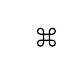
\begin{tikzpicture}[yshift=-0.15ex,menukeys key symbol]
         \draw (0.5ex,0.7ex) -- (0.5ex,1.25ex) arc (0:270:0.25ex) -- %
               (1.25ex,1ex) arc (-90:180:0.25ex) -- (1ex,0.25ex) %
               arc (-180:90:0.25ex) -- (0.25ex,0.5ex) arc (90:360:0.25ex) %
               -- cycle;
      \end{tikzpicture}%
   }%
}
\tw@make@key@macro*{\cmd}
%    \end{macrocode}
% \end{macro}
% \begin{macro}{\Space}\begin{macro}{\SPACE}
%    \begin{macrocode}
\providecommand*{\Space}{\expandonce{\rule{3em}{0pt}}}
\newcommand{\spacename}{Space}
\providecommand*{\SPACE}{\expandonce{\rule{2em}{0pt}\spacename\rule{2em}{0pt}}}
%    \end{macrocode}
% \end{macro}\end{macro}
% \begin{macro}{\return}
%    \begin{macrocode}
\tw@make@key@box{return@mac}{%
   \begin{tikzpicture}[yshift=0.25ex,menukeys key symbol]
      \draw [->, rounded corners=0.2ex] (1.25ex,1ex) -| %
            (2ex,0) -- (0,0);
   \end{tikzpicture}%
}
\tw@make@key@box{return@win}{%
   \begin{tikzpicture}[menukeys key symbol]
      \draw [->] (1ex,1.25ex) |- (0,0);
   \end{tikzpicture}%
}
\tw@make@key@macro*{\return}
%    \end{macrocode}
% \end{macro}
% \begin{macro}{\enter}
%    \begin{macrocode}
\def\tw@mk@enter@win{Enter}
\tw@make@key@box{enter@mac}{%
   \begin{tikzpicture}[menukeys key symbol]
      \draw (0,0) -- (0.5ex,0.5ex) -- (1ex,0);
      \draw (0,0.55ex) -- (1ex,0.55ex);
   \end{tikzpicture}%
}
\tw@make@key@macro*{\enter}
%    \end{macrocode}
% \end{macro}
% \begin{macro}{\winmenu}
%    \begin{macrocode}
\def\tw@mk@winmenu@mac{%
   \tw@mk@warning{'\string\winmenu' only for Windows!}%
}
\tw@make@key@box{winmenu@win}{%
   \begin{tikzpicture}[yshift=-0.2ex,menukeys key symbol]
      \draw (0,0) rectangle (1.5ex,1.8ex);
      \draw (0.25ex,1.4ex) -- ++(1ex,0);
      \draw (0.25ex,1ex) -- ++(1ex,0);
      \draw (0.25ex,0.6ex) -- ++(1ex,0);
   \end{tikzpicture}%
}
\tw@make@key@macro*{\winmenu}
%    \end{macrocode}
% \end{macro}
% \begin{macro}{\backspace}
%    \begin{macrocode}
\tw@make@key@box{backspace}{%
   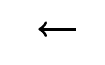
\begin{tikzpicture}[yshift=0.65ex,menukeys key symbol]
      \draw [<-,menukeys thick] (0,0) -- (1.35em,0);
   \end{tikzpicture}%
}
\tw@make@key@macro{\backspace}
%    \end{macrocode}
% \end{macro}
% \begin{macro}{\del}\begin{macro}{\backdel}
% \changes{v1.4}{2016/04/17}{Added \cs{backdel}}
%    \begin{macrocode}
\providecommand{\delname}{Del.}
\def\tw@mk@del@win{\delname}
\tw@define@mackey{%
   \def\tw@mk@del@mac{\delname}%
}{%
   \tw@make@key@box{del@mac}{%
      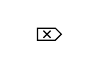
\begin{tikzpicture}[yshift=0.2ex,menukeys key symbol]
         \draw (0,0) -- (1.5ex,0) -- (2ex,0.5ex) --%
               (1.5ex,1ex) -- (0,1ex) -- cycle;
         \draw (0.5ex,0.2ex) -- (1.1ex,0.8ex);
         \draw (0.5ex,0.8ex) -- (1.1ex,0.2ex);
      \end{tikzpicture}%
   }%
}
\tw@make@key@macro*{\del}
\def\tw@mk@backdel@win{\delname}
\tw@define@mackey{%
   \def\tw@mk@backdel@mac{\delname}%
}{%
   \tw@make@key@box{backdel@mac}{%
      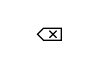
\begin{tikzpicture}[yshift=0.2ex,menukeys key symbol]
         \draw (2ex,0) -- (0.5ex,0) -- (0,0.5ex) --%
               (0.5ex,1ex) -- (2ex,1ex) -- cycle;
         \draw (1ex,0.2ex) -- (1.6ex,0.8ex);
         \draw (1ex,0.8ex) -- (1.6ex,0.2ex);
      \end{tikzpicture}%
   }%
}
\tw@make@key@macro*{\backdel}
%    \end{macrocode}
% \end{macro}\end{macro}
%
% \begin{macro}{\arrowkeyup}\begin{macro}{\arrowkeydown}
% \begin{macro}{\arrowkeyleft}\begin{macro}{\arrowkeyright}
% Lastly we define the arrow macros:
%    \begin{macrocode}
\tw@make@key@box{arrowkeyup}{%
   \begin{tikzpicture}[yshift=-0.2ex,menukeys key symbol]
      \draw [->] (0,0) -- (0,0.8em);
   \end{tikzpicture}%
}
\tw@make@key@macro{\arrowkeyup}

\tw@make@key@box{arrowkeydown}{%
   \begin{tikzpicture}[yshift=0.7em,menukeys key symbol]
      \draw [->] (0,0) -- (0,-0.8em);
   \end{tikzpicture}%
}
\tw@make@key@macro{\arrowkeydown}

\tw@make@key@box{arrowkeyright}{%
   \begin{tikzpicture}[yshift=0.5ex,menukeys key symbol]
      \draw [->] (0,0) -- (0.8em,0);
   \end{tikzpicture}%
}
\tw@make@key@macro{\arrowkeyright}

\tw@make@key@box{arrowkeyleft}{%
   \begin{tikzpicture}[yshift=0.5ex,menukeys key symbol]
      \draw [->] (0,0) -- (-0.8em,0);
   \end{tikzpicture}%
}
\tw@make@key@macro{\arrowkeyleft}
%    \end{macrocode}
% \end{macro}\end{macro}\end{macro}\end{macro}
% \begin{macro}{\arrowkey}
% And the |\arrowkey| macro that get's it's direction as argument.
%    \begin{macrocode}
\newcommand{\arrowkey}[1]{%
   \IfStrEq{^}{#1}{\arrowkeyup}{%
      \IfStrEq{v}{#1}{\arrowkeydown}{%
         \IfStrEq{<}{#1}{\arrowkeyleft}{%
            \IfStrEq{>}{#1}{\arrowkeyright}{%
               \tw@mk@error{Wrong value '#1' for \string\arrowkey\MessageBreak
               Possible values are '^', 'v', '<' or '>'}%
            }%
         }%
      }%
   }%
}
%    \end{macrocode}
% \end{macro}
% Close the |\iftw@mk@definekeys|
%    \begin{macrocode}
\fi
%    \end{macrocode}
%
%
% \Finale
\endinput